\documentclass[a4paper]{article}
\usepackage[utf8]{inputenc}
\usepackage[english,russian]{babel}

\ifx\pdfoutput\undefined
\usepackage{graphicx}
\else
\usepackage[dvips]{graphicx}
\fi

\usepackage{setspace}
 \setlength{\parskip}{1ex}
 \setlength{\topmargin}{0in}
 \setlength{\oddsidemargin}{0in}
 \setlength{\evensidemargin}{0in}
 \setlength{\textheight}{9in}
 \setlength{\textwidth}{6.25in}
% \setlength{\headwidth}{6.25in}

\begin{document}

\author{Иван Антонюк, Мансур Зиятдинов, Евгений Кацевман, Роман Кириллов}
\title{Dreamantle Robotix}
\maketitle


\section{Основные расходные материалы}
\begin{itemize}
\item EeePC 701
\item usb камера dns
\item машинка на радиоуправлении
\item cArduino Nano v4
\item беспайная макетка
\item кусок фанеры
\item два сервопривода hxt900
\item аккумулятор
\item уголки
\item шурупы
\item геймпад
\item микросхема l298n
\end{itemize}

\section{Общие сведения}
На шасси от игрушечной машинки стоит ноутбук, который по USB отправляет команды на Arduino. Ардуино управляет двигателями и сервомашинками.
Команды на ноут принимаются через ssh по wi-fi. По wi-fi же идет трансляция видео с камеры (сейчас просто через X11). Сложные вычисление планируется производить на головной машине, а обратно на ноут отпралять результаты и команды.
Исходные коды прилагаются к этому документу.

\section{Аппаратная часть}

\subsection{Схема включения arduino}
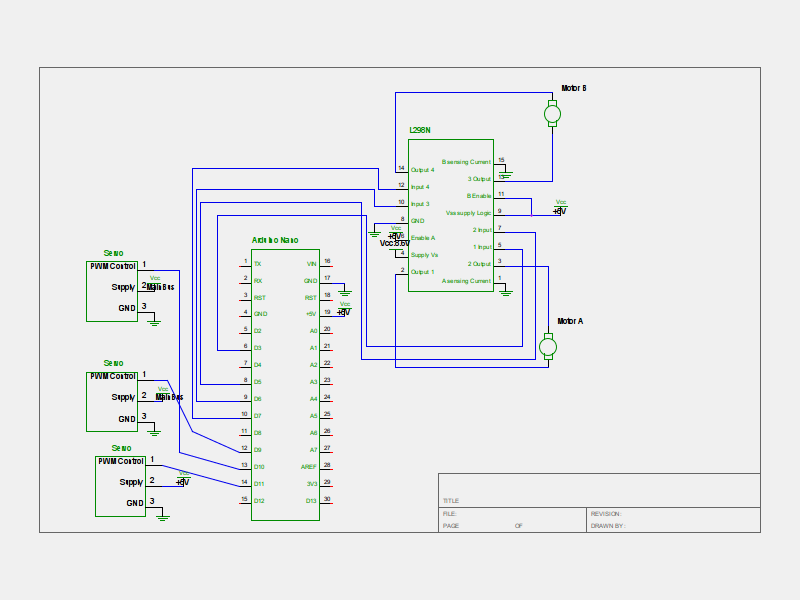
\includegraphics[keepaspectratio, width=15cm]{rt1cotton.eps}
 
У сервоприводов hxt900 три провода - земля, питание и сигнал. Земля подключена к общей земле, питание к 5V Arduino (получается, что они питаются от USB), а сигналы к 9, 10 и 11 ногам (ШИМ).
Маршевый и рулевой моторы включены через драйвер L298N. 1 и 15 ноги драйвера (current sensing) заземлены, 2 и 3 (output1 и output2) подключены к маршевому двигателю, нога 4 драйвера к общему питанию, 5 и 7 (input1 и input2) к 3 и 5 ногам Arduino (ШИМ, управление маршевым двигателем), 6(Enable A) к 5V Arduino, 8 заземлена 9 к 5V Arduino , 10 и 12 (input 3 и input 4) к 6 и 7 ногам Arduino (Руление, без ШИМ), 11 к 5V Arduino, 13 и 14 (output3, output4) к рулевому мотору.   

Маршевый и рулевой моторы питаются от отдельного 9-вольтового модельного аккумулятора на 1200 мАч.

\section{Прошивка Arduino}
Текст прошивки находится в файле car3.pde.

В Ardino прошит простой интерпретатор, который получает с UART текстовые команды и сразу выполняет их. Длина команд с параметрами ограничена 20 символами. Список выполняемых команд:
\begin{description}
\item[h X] повернуть камеру по горизонтали в направлении X, где X --- число градусов от 0 до 180. h 90 устанавливает камеру по центру
\item[v X] то же самое, но в вертикальном направлении
\item[on] включить светодиод
\item[off] выключить светодиод
\item[s X] повернуть рулевые колеса в направлении X (0-180)
\item[e X] установить направление и мощность для маршевого мотора. X=90 --- стоп, X=180 --- полный вперед, X=0 --- полный назад.
\end{description}

Каждая команда сейчас может принимать один числовой параметр. Список команд перечислен в массиве mapping. Ниже приведены описание mapping и одна из выполняемых функций.
\begin{verbatim}

void ledOn(int){
  digitalWrite(LEDPIN, HIGH);
}

typedef struct {
  char cmd[20];
  void (&action)(int);
} mapentry;


mapentry mapping[]={{"on",ledOn},
			     {"off",ledOff},
			     {"full",full},
			     {"h",goH},
			     {"v",goV},
			     {"e",goE},
			     {"s",goS}};
\end{verbatim}

Чтобы добавить свои команды, нужно написать выполняющие их функции и расширить mapping.

\section{Управление}
\subsection{Отправка команд Arduino}
Arduino виден с компьютера как символьное устройство (/dev/ttyUSB0 или с похожим названием). В него можно писать и из него можно читать штатными средствами операционной системы. Т.к. прошивка рассчитана на работу с текстовыми командами, то простую программу можно написать даже на cmd/bash.

В самом начале работы нужно правильно настроить порт:
\begin{verbatim}
stty -F $1 ispeed 115200 ospeed 115200 line 0 eof ^A 
    min 0 time 0 -brkint -icrnl -imaxbel -onlcr 
    -isig -icanon -iexten -echo -echoe -echok -echoctl -echoke -opost
\end{verbatim}

Нужно обязательно слушать, что отвечает Arduino, поэтому в фоне запускаем tail:
\begin{verbatim}
tail -f /dev/ttyUSB0 &
\end{verbatim}

После этого можно отправлять команды.
\begin{verbatim}
echo on >>/dev/ttyUSB0
echo v 90 >>/dev/ttyUSB0
\end{verbatim}

\subsection{Трансляция видео}

\subsubsection{X11}
Самый простой и быстрый для выполнения вариант --- сделать трансляцию видео по X11 через ssh, например, запустив mplayer на нетбуке.

\begin{verbatim}
ssh -X 10.42.43.11 "mplayer tv:// -tv width=160:device=/dev/video0"
\end{verbatim}

\subsubsection{mjpg-streamer}
В данный момент видео транслируется с помощью mjpg-streamer (http://sourceforge.net/projects/mjpg-streamer). Поток можно ловить на управляющей машине с помощью OpenCV, быстро обрабатывать, и отправлять обратно команды.

Команда для поднятия mjpg-streamer:

\begin{verbatim}
LD_LIBRARY_PATH=./ ./mjpg_streamer -i "input_uvc.so -d /dev/video0 -r 160x120 -f 30 -y -q 90" -o "output_http.so -p 8080 -n"
\end{verbatim}

Запускать её нужно из той директории, где был скомпилирован mjpg-streamer.
\subsection{Управление с геймпада}

Для работы с геймпадом написан скрипт на Python с библиотекой pygame. Скрипт слушает события с джойстика, и регулярно пишет в стандартный вывод полное состояние джойстика в формате команд Arduino (см. выше).
Скрипт находится в файле joystick.py.

Команды передаются через пайп c ssh с cat >>/dev/ttyUSB0 на том конце:
\begin{verbatim}
python -u joystick2.py | ssh 10.42.43.11 "cat >>/dev/ttyUSB0" 
\end{verbatim}
-u нужен, чтобы python не буферизовал вывод, а печатал все сразу.

Скрипты для запуска всего --- clientstart.sh и start.sh --- находятся в этом же архиве.

\end{document}



\bye 
